%\documentclass[a4paper,handout]{beamer}
\documentclass[presentation]{beamer}
\usepackage[english]{babel}
\usepackage[utf8]{inputenc}
\usetheme{Inuits}
\usepackage[T1]{fontenc}
\usepackage{listings}
\usepackage{hyperref}
\usepackage{eso-pic}
\setbeamercolor{background canvas}{bg=}
\definecolor{inuitstitle}{RGB}{153,153,255}
\definecolor{inuitsgreen}{RGB}{35,255,35}
\usecolortheme[RGB={90,90,149}]{structure}
\usebackgroundtemplate{%
\includegraphics[height=\paperheight,width=\paperwidth]{files/background.png};}

%\AddToShipoutPicture{\put(0,5){%
%   \parbox[b][\paperheight]{\paperwidth}{%
%     \vfill
%     \centering
%     \rotatebox{0}{\includegraphics[width=\paperwidth,height=\paperheight,%
%                      ]{files/background.png}}%
%     \vfill
%}}}
\setbeamercolor{normal text}{fg=white}
\setbeamercolor{block body}{fg=black}
\setbeamercolor{itemize item}{fg=inuitsgreen}
\setbeamercolor{itemize subitem}{fg=inuitsgreen}
\setbeamercolor{itemize subitem subitem}{fg=inuitsgreen}
\setbeamertemplate{itemize item}[circle]
\setbeamertemplate{itemize subitem}[circle]
\setbeamertemplate{sections/subsections in toc}[circle]

%\setbeamercolor{palette primary}{fg=inuitstitle,bg=black!85}
%\setbeamercolor{palette secondary}{fg=white,bg=inuitstitle}
%\setbeamercolor{palette tertiary}{fg=white,bg=black!85}
%\setbeamercolor{palette quaternary}{fg=inuitstitle}
%\setbeamercolor{block title}{fg=inuitstitle}
%\setbeamercolor{sidebar}{bg=inuitstitle!70}

%\AtBeginDocument{%
%    \pgfdeclareverticalshading{beamer@topshade}{\paperwidth}{%
%      color(0pt)=(bg);
%      color(4pt)=(black)}
%}


\setbeamercolor{title}{fg=inuitstitle,bg=}

\setbeamertemplate{navigation symbols}{}
\definecolor{OliveGreen}{RGB}{0,100,0}
\definecolor{grey}{RGB}{150,150,150}
\begin{document}
\setbeamercovered{invisible}
\title[Deployment orchestration]{\fontsize{30}{35}\selectfont Deployment orchestration}
\author{Jan Collijs}
\institute[Inuits]{\includegraphics[height=2cm]{files/inuitslogo.png}}
\date{\today}

\frame[plain]{\titlepage}

\frame{%
\frametitle{Table of contents}
\tiny
\tableofcontents
}

\section{Introduction}
\subsection{whoami}
\frame{%
	\frametitle{Profile}
	Sysadmin \\
	Linux \& Open-Source enthusiast\\
	Consultant for \href{https://inuits.eu}{inuits.eu}\\
	\medskip
	\href{https://twitter.com/visibilityspots}{@visibilityspots}\\
}

\section{Background}

\subsection{project}
\frame{%
	\frametitle{University library of Ghent}
	\begin{itemize}
		\item{5 developers}
		\item{devops integration}
		\item{New website}
		\item{2 environments: dev/prod}
	\end{itemize}
}

\subsection{versioning}
\frame{%
	\frametitle{Versioning}
	\begin{itemize}
		\item{Software code is based into a repository}
		\item{History of changes is available}
		\item{Collaboration}
		\item{Hooks}
		\item{Many tools available (git, redmine, gitlab, chili project, \ldots)}
	\end{itemize}
}

\subsection{continuous integration}
\frame{%
	\frametitle{Jenkins}
	\begin{itemize}
		\item Automation tool
		\item Triggered by hooks
		\item Custom scripts
	\end{itemize}
}

\frame{%
	\frametitle{Jenkins flow example}
	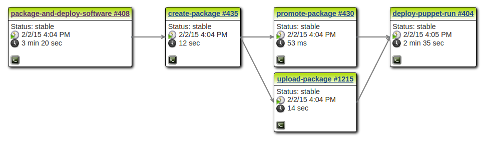
\includegraphics[height=3cm]{files/flow.png}
}

\subsection{packaging}
\frame{%
	\frametitle{fpm/rpmbuild}
	\begin{itemize}
		\item \href{https://github.com/jordansissel/fpm}{fpm}
		\item \href{http://www.rpm.org/max-rpm/s1-rpm-build-creating-spec-file.html}{spec file}
		\item \href{http://www.rpm.org/max-rpm-snapshot/rpmbuild.8.html}{rpmbuild}
	\end{itemize}
}

\subsection{repository management}
\frame{%
	\frametitle{Yum-repo-server}
	\begin{itemize}
		\item Repository management
		\item One repository per environment (dev/prod)
		\item Only used for own software
		\item \href{https://github.com/visibilityspots/vagrant-yum-repo-server}{Vagrant setup}
	\end{itemize}
}

\section{Configuration management}
\subsection{puppet}
\frame{%
	\frametitle{Puppet}
	\begin{itemize}
		\item Configures ALL servers and services
		\item Hiera
		\item Roles \& profiles
		\item Custom module for every piece of software
		\item Cron based runs
	\end{itemize}
}

\subsection{puppetdb}
\frame{%
	\frametitle{Puppetdb}
	\begin{itemize}
		\item Consists puppet data (postgresql DB)
		\item Query API (experimental v4)
	\end{itemize}
}

\begin{frame}[fragile]
\frametitle{Query puppetdb}
\scriptsize\begin{verbatim}
# Look up the nodes which have the given resource type and name declared
for NODE in $(curl --silent -G https://PUPPETDB_HOST:PUPPETDB_PORT/v4/ \
environments/ENVIRONMENT/resources/TYPE/RESOURCENAME | grep certname | \
 awk -F ':' '{print $2 }' | cut -d '``' -f2)
do
  nodes=(''${nodes[@]}" $NODE)
done
\end{verbatim}
\end{frame}

\section{Orchestration}
\subsection{ansible}
\frame{%
	\frametitle{Ansible}
	\begin{itemize}
		\item Based on ssh
		\item No agent on the servers
		\item User on the clients with public key and sudo rights
	\end{itemize}
}

\frame{%
	\frametitle{Dynamic inventory script}
	\begin{itemize}
		\item Static inventory
		\item Dynamic inventory (\href{https://github.com/visibilityspots/ansible-puppet-inventory}{https://github.com/visibilityspots/ansible-puppet-inventory})
		\item Pypuppetdb lib (\href{https://github.com/puppet-community/pypuppetdb/pull/34}{https://github.com/puppet-community/pypuppetdb/pull/34})
		\item Dynamic inventory ansible core (\href{https://github.com/ansible/ansible/pull/9593}{https://github.com/ansible/ansible/pull/9593})
	\end{itemize}
}

\subsection{automation}
\frame{%
	\frametitle{Deploy puppet run}
	\begin{itemize}
		\item Jenkins
		\item puppet-check script (\href{https://github.com/visibilityspots/ci-scripts/blob/master/puppet/puppet-check.sh}{https://github.com/visibilityspots/ci-scripts/blob/master/puppet/puppet-check.sh})
	\end{itemize}
}

\begin{frame}[fragile]
\frametitle{Code}
\begin{verbatim}
for NODE in "${nodes[@]}"
do
  echo "Process $NODE:"
  echo ""
  ansible $NODE -a "puppet agent --test" --sudo;
  echo "======================================="
done
\end{verbatim}
\end{frame}

\frame{%
	\frametitle{Console output}
	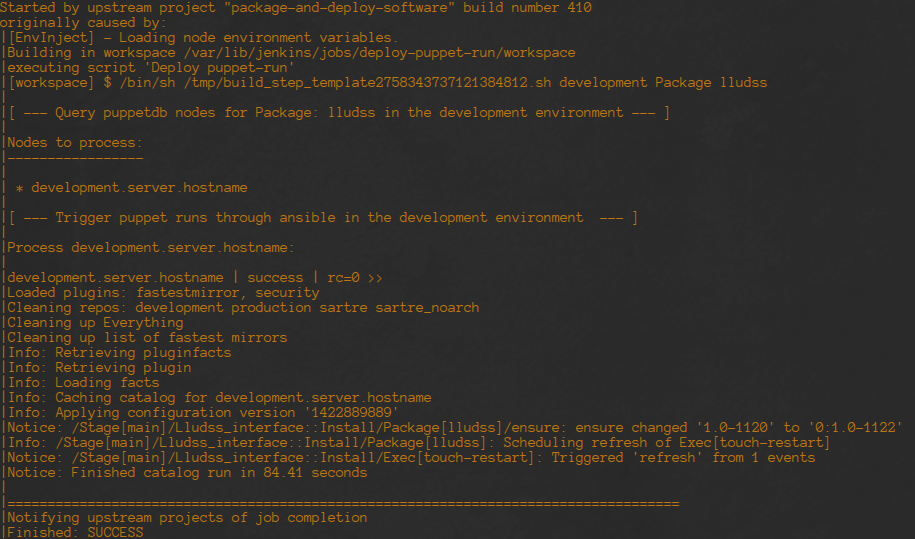
\includegraphics[height=8cm]{files/console.png}
}

\subsection{online-material}
\frame{%
	\frametitle{online material}
	\begin{itemize}
		\item \href{http://visibilityspots.com/ansible-orchestration.html}{http://visibilityspots.com/ansible-orchestration.html}
		\item \href{https://github.com/visibilityspots/ansible-puppet-inventory}{https://github.com/visibilityspots/ansible-puppet-inventory}
		\item \href{https://github.com/visibilityspots/ci-scripts}{https://github.com/visibilityspots/ci-scripts}
	\end{itemize}
}

\section{Questions}
\frame{%
	\frametitle{Questions}
	
\includegraphics[height=6cm]{files/questions.jpg}
}

\end{document}
